\documentclass{article}
% All latex files should begin with a "documentclass" declaration.

% By the way, the "comment character" in latex is the percent sign.  So, anything after a % on a line will be ignored when compiling the source document.  We'll use that a lot, and you may want to use it to leave yourself notes as you're learning.  A good text editor will display comments in a different color or font, so that it's obvious what is latex and what is notes.

% All latex commands begin with a backslash, \.  Curly braces { } contain mandatory arguments to a command.  Square brackets [ ] contain optional arguments.

% For example, try editing the first line to read instead:\documentclass[12pt]{article}
% Providing that optional argument to the documentclass command changes the font size from the default (10 point) to 12 point.

% Here is much more (totally optional) information about documentclass: http://texblog.org/2013/02/13/latex-documentclass-options-illustrated/

%%%%%%%%%%%%%%%%
%%% PREAMBLE %%%
%%%%%%%%%%%%%%%%

% The preamble is a set of formatting instructions, which you provide to latex before your actual content.  It begins with the \documentclass command, above.  Then typically a lot of packages are loaded, and maybe some other declarations.  All of that can be typed right here.

% Alternatively, it can be helpful to confine much of the preamble to a separate file.  This keeps it out of your way and makes it easy to reuse for other documents.  Here, I've put most of the preamble into a separate file, which we'll load now:
\usepackage{tutorial}  % loads the tutorial.sty file
% You can take a look in tutorial.sty now, and we'll refer to it later on.

% But just to illustrate that formatting commands can be given here in the main document, try uncommenting one of these next lines (that is, remove the comment % from the beginning of the line).  This will change the font throughout the document, from LaTeX's classic Computer Modern to something else.
%
%\usepackage{mathptmx}     % Times font, for text and math
%\usepackage[sc]{mathpazo} % snazzy font suggested by American Naturalist

\title{Yet Another \LaTeX\ Tutorial}
\author{For Foundations Class}
\date{2 December 2015}

\begin{document} %  Essential!  And don't forget the matching \end{document} at the end of your content.

\maketitle
% This goes with the \title{} above.  There is lots more about titlepages here: https://en.wikibooks.org/wiki/LaTeX/Title_Creation

%%%%%%%%%%%%%%%%%
%%% MAIN TEXT %%%
%%%%%%%%%%%%%%%%%

Each section below highlights features or commands in \LaTeX.
Each ends with a suggestion for experimenting with what you've just learned.
Definitely feel free to experiment more!

%--------------------------------------------------
\section{Paragraphs}
\label{sec:paragraphs}
%--------------------------------------------------

Paragraphs are separated by blank lines in the source file.
If there is no blank line, the text is all formatted as the same paragraph.
Thus, \LaTeX\ ignores the linebreak that comes at the end of each sentence here.
One sentence per line is good practice, though, especially when using version control (like \texttt{git}).

Here is the start of a new paragraph.  \\
The double-backslash causes this sentence to start on a new line, but without a paragraph break.

\vspace{20pt}
Adding more blank lines doesn't increase the amount of space between paragraphs.
To do that, we use the \latexcode{\\vspace} command to add a specified amount of vertical space.

Here are some miscellaneous examples of text formatting.
\textbf{Bold.}
\emph{Emphasized.  Usually italic.  But can be un-italicized if \emph{emphasized} within italics.}
\large{Larger than usual.}
\small{Smaller than usual.}
`Inside single smart quotes.'
``Inside double smart quotes---it's an em-dash!''

\subsection{\task}

Write two paragraphs of text.
Try to stick with one line per sentence.
Use unnecessary text formatting (bold, etc.)

Adjust the paragraph indentation and spacing between paragraphs by changing the values of \latexcode{\\parindent} and \latexcode{\\parskip} in \latexcode{tutorial.sty}.

Notice how nice the justified text looks.
But to remove the right justification, find the \latexcode{\\raggedright} command in \latexcode{tutorial.sty}.

%--------------------------------------------------
\section{Custom Commands}
\label{sec:custom}
%--------------------------------------------------

Now let's jump straight to an advanced \LaTeX\ feature: defining your own commands.
We've already used two of them, which I put into \latexcode{tutorial.sty}.
One is \latexcode{\\latexcode}, for printing \LaTeX\ commands without executing them---it's a bit complicated, so don't mess with that line.

\subsection{\task}

The other custom command is simpler, and you can easily change it.
I wanted each subsection of exercises to have the same name, but I kept changing my mind about what that name should be.
It is currently \task.
Go into \latexcode{tutorial.sty}, find the line where \latexcode{\\task} is defined, and change the definition to something else, maybe ``Exercises'' or ``Tasks''.
Now notice the new name of this subsection, and of all the other ones with tasks.
This is a handy trick to maintain consistency without repeated bouts of search-and-replace.

%--------------------------------------------------
\section{Sections}
\label{sec:sections}
%--------------------------------------------------

We have also defined in \latexcode{tutorial.sty} how the section headings should look, using the \latexcode{titlesec} package.

\subsection{This is a Subsection}

\subsubsection{This is a Subsubsection}

\subsubsection*{This is a Subsubsection Without a Number}

We can refer to sections by number, even if we don't know what the number is.
For example, we discussed custom commands in \cref{sec:custom}, and we are now discussing sections in \cref{sec:sections}.
We'll talk about cross-referencing more below (\cref{sec:refs}), but for now, just know that the key was the \latexcode{\\label} command we issued right after the name of each section.

\subsection{\task}

In \latexcode{tutorial.sty}, change the subsubsection format to small caps.
Look at the lines above to check that it worked.

Refer by number to the section where we discussed paragraph formatting.

%--------------------------------------------------
\section{Math}
\label{sec:math}
%--------------------------------------------------

Math typesetting is where \TeX\ shines.
Inline math is denoted with \latexcode{\$}.
For example, $\alpha_z = 1$ but $\Gamma^2 = \sqrt{7 y}$.

Display math works like this:
\begin{equation}
    \frac{d}{dx} \left( \int_{0}^{x} f(u)\, du \right) = f(x)
\label{eq:deriv}
\end{equation}

% Here is a ton more info on math typesetting:
%     https://en.wikibooks.org/wiki/LaTeX/Mathematics
%     http://mirrors.ctan.org/macros/latex/required/amslatex/math/amsldoc.pdf

\section{\task}

The quadratic equation is
\begin{equation}
    a x^2 + b x + c = 0.
\label{eq:quadratic}
\end{equation}
Write out its solution for x.
% Hint: https://en.wikipedia.org/wiki/Quadratic_formula

%--------------------------------------------------
\section{Figures}
\label{sec:figures}
%--------------------------------------------------

explain about floats

\begin{figure}[h]
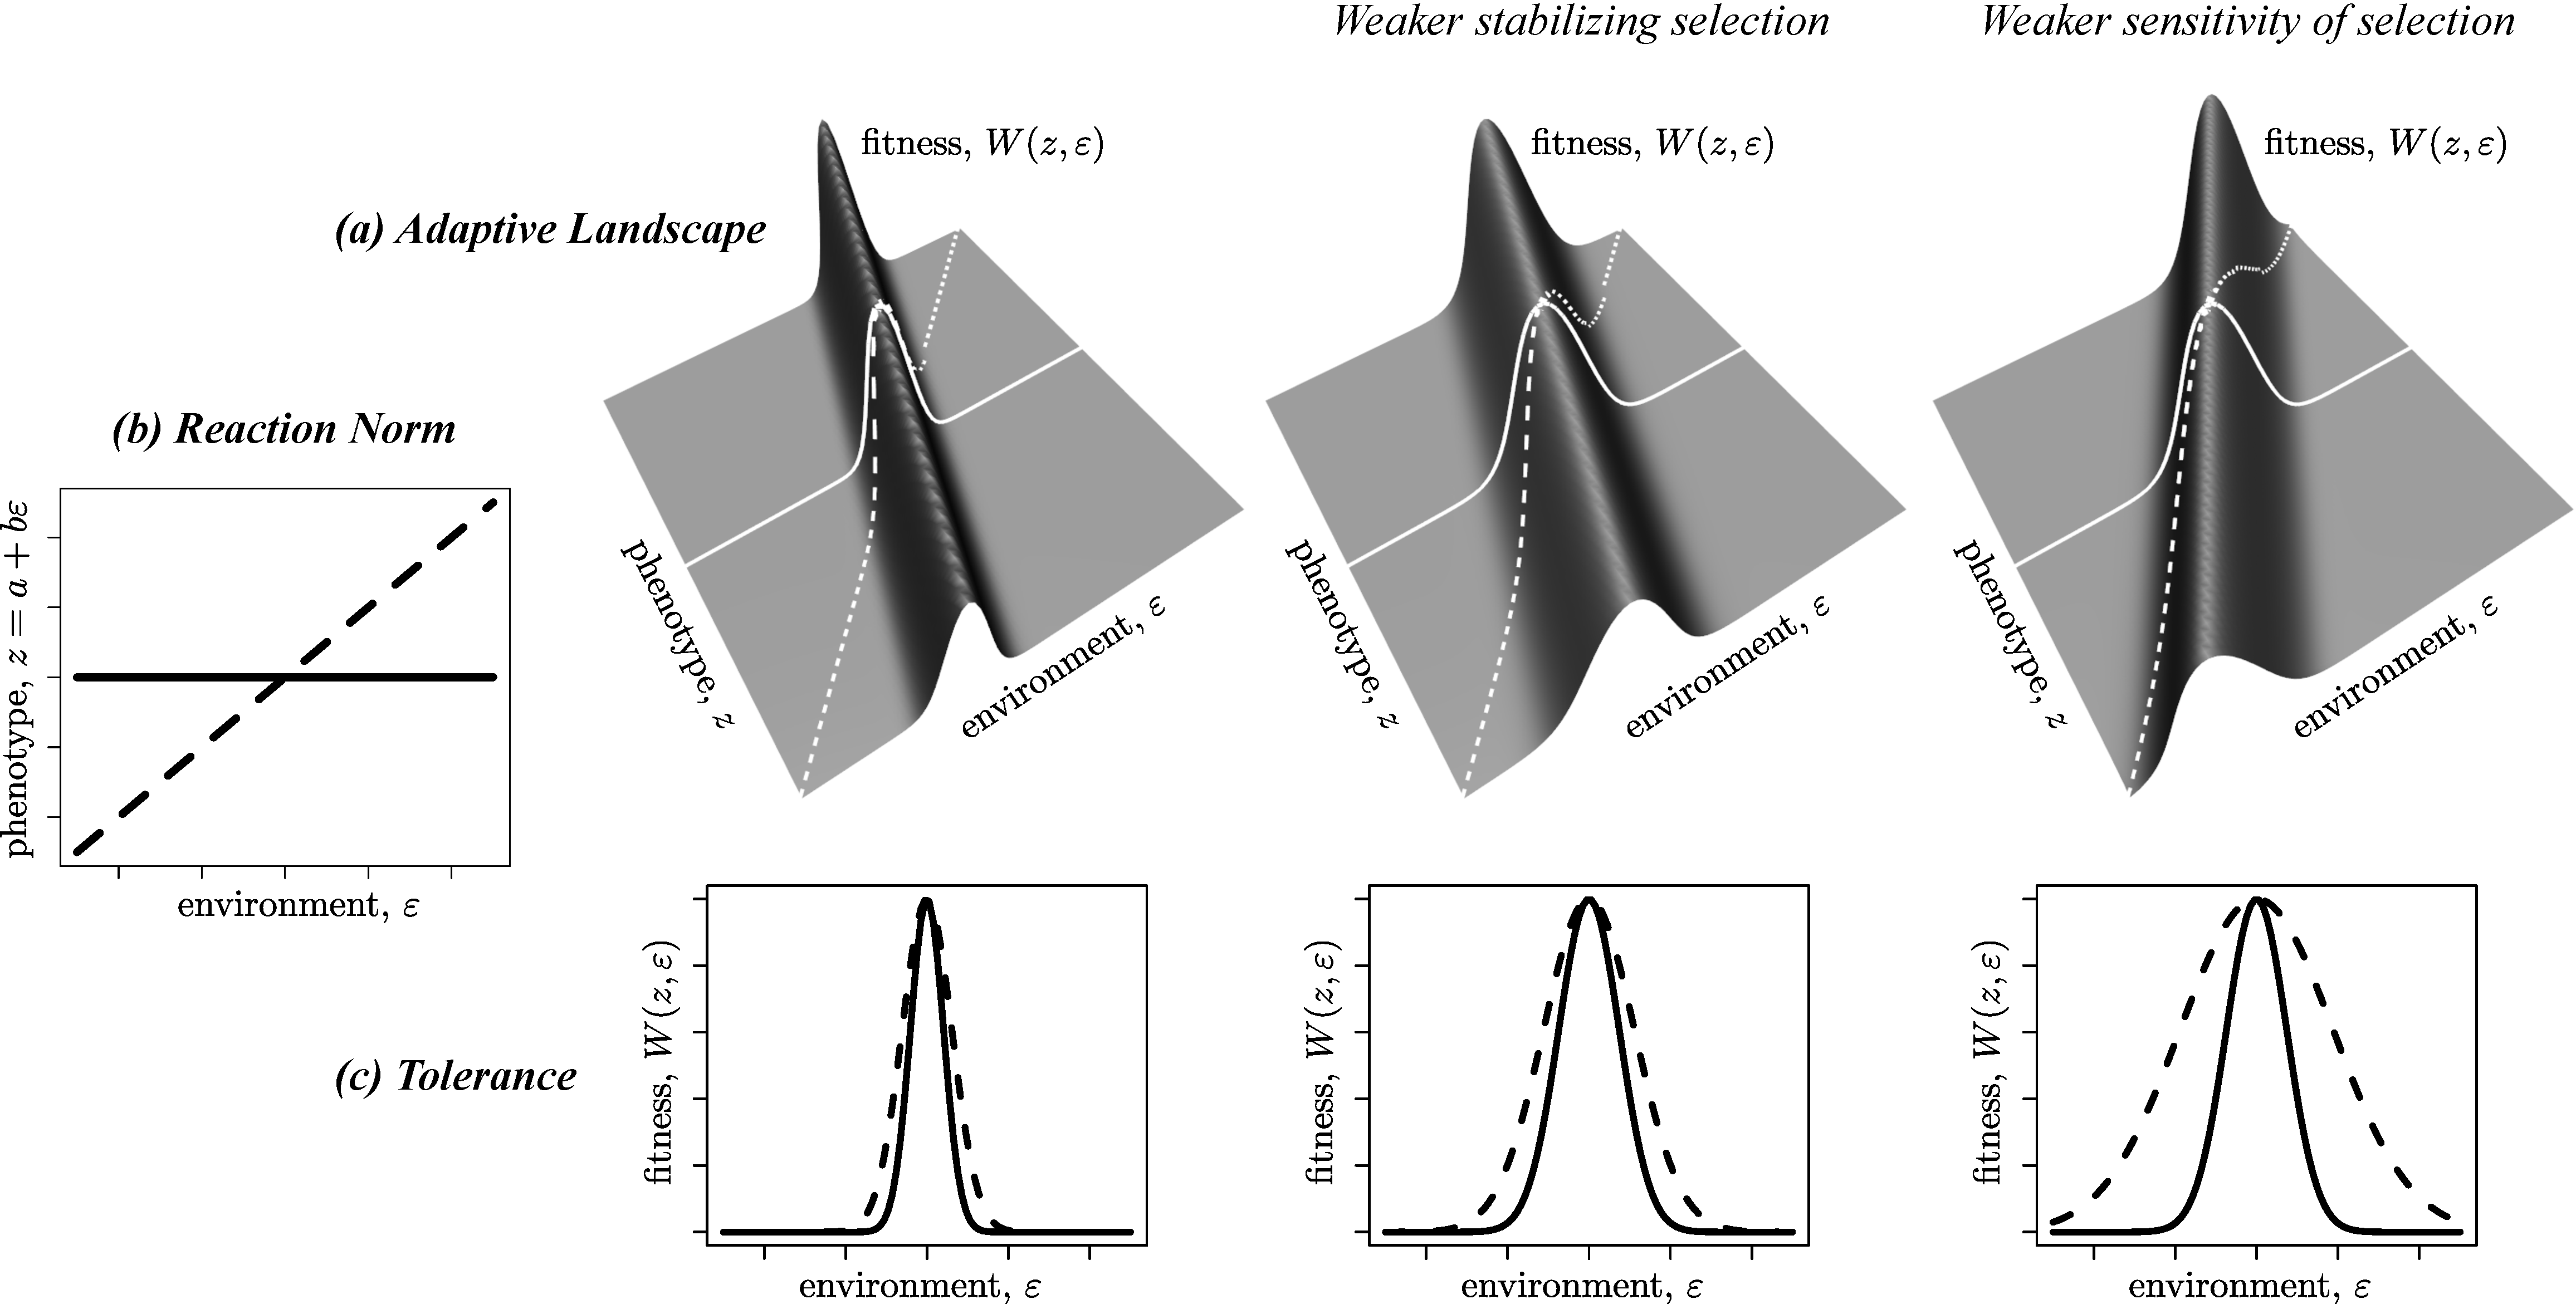
\includegraphics[width=0.9\textwidth]{landscape.pdf}
\caption{A generalized adaptive landscape.
    This is here because it was the first PDF figure I found.
    \LaTeX\ can handle lots of graphics formats, but PDF is especially nice because it is a vector format and so scales well.
    By the way, Inkscape is fantastic (and free) software for making vectorized figures and diagrams.
}
\label{fig:landscape}
\end{figure}

\begin{SCfigure}[50]
\centering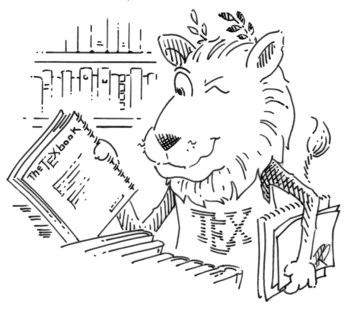
\includegraphics[width=0.25\textwidth]{lion.png}
% https://www.ctan.org/lion/
\caption{CTAN lion drawing by Duane Bibby.
    Also, this caption is to the side of the image.
    Non-standard, but sometimes useful.
}
\label{fig:lion}
\end{SCfigure}

\TeX\ has a classy mascot, as we see in \cref{fig:lion}.
There is also some biology in \cref{fig:landscape}.

a note about figure placement \\
endfloat: move all figures to end

%--------------------------------------------------
\section{Cross-Referencing}
\label{sec:refs}
%--------------------------------------------------
% TODO

cref \\
section by name (number was done above) \\
equation, figure, table \\
change Figure to Fig.


\end{document} % Essential!  The end of your content.


If using Overleaf (preliminaries)
    write down url
    switch to Manual
    create Version
    open Projects panel to see files
    panel to edit source file, panel to see compiled pdf
    git clone (just fyi; won't use here)

lists

(use booktabs)
tabular
table (floating env)
copy, add row, add column, align column
(R's xtable)

\include table or some text

bibliography
bibtex, biblatex

line numbers

table of contents
